\begin{center}
\indent
\textit{La loro teoria serve ad inquadrare la risoluzione dei problemi lineare. Spazio vettoriale delle matrici, spazio vettoriale delle $n$-uple di numeri reali.}
\end{center}

Gli spazi vettoriali reali sono particolari strutture algebriche sui reali $\mathbb{R}$ con due operazioni $\left( V, +, \cdot \right)$ dove + \`e la classica operazione binaria $+ : V \times V \to V$, mentre $\cdot$ \`e un'operazione ``esterna'' $\cdot : \mathbb{R} \times V \to V$. Gli elementi di $V$ si dicono \textit{vettori}.

\section{Propriet\`a degli spazi vettoriali}

\begin{enumerate}
    \item $\left ( V, + \right )$ \`e un gruppo abelliano.
    \item $ \cdot : \mathbb{R} \times V \to V $ \`e un'operazione associativa. $ r, s \in \mathbb{R}, \ v \in V : \left( r \cdot s \right ) \cdot v = r \cdot (s \cdot v) = s \cdot (r \cdot v)$
    \item Propriet\`a distributiva rispetto all'addizione vettoriale: $ r \in \mathbb{R}, v, w \in V : r \cdot (v + w) = r \cdot v + r \cdot w$
    \item $ \forall r, s \in \mathbb{R} : (r + s) \cdot v = r \cdot v + s \cdot v $
    \item $1 \cdot v = v$
\end{enumerate}

$V =$ insieme dei vettori geometrici del piano applicati in $O$.

$+ : V \times V \to V$

La somma si effettua con la ``regola del parallelogramma'' (figura \ref{fig:parallelogramma}). Le forze possono essere rappresentate dai vettori del piano.

\begin{figure}[ht]
\centering
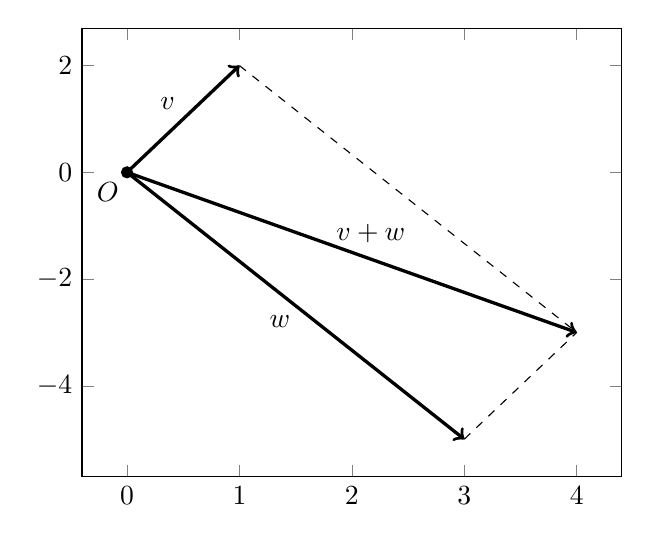
\begin{tikzpicture}
\begin{axis}[
    % graph options
]
\addplot [black, mark = *, nodes near coords=$O$,every node near coord/.style={anchor=45}] coordinates {( 0, 0)};
\addplot [black, nodes near coords=$v$,every node near coord/.style={anchor=315}] coordinates {( 0.5, 1)};
\addplot [black, nodes near coords=$w$,every node near coord/.style={anchor=45}] coordinates {( 1.5, -2.5)};
\addplot [black, nodes near coords=$v+w$,every node near coord/.style={anchor=225}] coordinates {( 2, -1.5)};
\addplot[very thick,->] coordinates {(0,0) (1,2)};
\addplot[very thick,->] coordinates {(0,0) (3,-5)};
\addplot[very thick,->] coordinates {(0,0) (4,-3)};
\addplot[dashed] coordinates {(1,2) (4,-3)};
\addplot[dashed] coordinates {(3,-5) (4,-3)};
\end{axis}
\end{tikzpicture}
\caption{\label{fig:parallelogramma}Metodo del parallelogramma}
\end{figure}

L'elemento neutro \`e il vettore nullo, i cui estremi coincidono in $O$, $\underline{\underline{O}} = \overrightarrow{OO}$. 

L'inverso di un vettore $v$ \`e chiamato $-v$, ha stessa direzione, stesso modulo e verso contrario.

Per creare lo spazio vettoriale abbiamo bisogno dell'operazione esterna: il prodotto scalare $ \cdot : \mathbb{R} \times V \to V$ (figura \ref{fig:prodotto_scallare}).

\begin{figure}[ht]
\centering
\begin{tikzpicture}
\begin{axis}[
    % graph options
]
\addplot [black, mark = *, nodes near coords=$O$,every node near coord/.style={anchor=135}] coordinates {( 0, 0)};
\addplot [black, nodes near coords=$v$,every node near coord/.style={anchor=315}] coordinates {( 0.5, 1)};
\addplot [black, nodes near coords=$-v$,every node near coord/.style={anchor=315}] coordinates {( -0.5, -1)};
\addplot [black, nodes near coords=$2v$,every node near coord/.style={anchor=135}] coordinates {( 1.5, 3)};
% \addplot[only marks] coordinates {(0,0)}; % punto
\addplot[very thick,->] coordinates {(0,0) (1,2)};
\addplot[dashed,->] coordinates {(0,0) (-1,-2)};
\addplot[dashed,->] coordinates {(0,0) (2,4)};
\end{axis}
\end{tikzpicture}
\caption{\label{fig:prodotto_scallare}Prodotto scalare}
\end{figure}

$(A, \cdot)$, $(B, \ast)$ due strutture algebriche. Possiamo costruire altre strutture algebriche, ad esempio sul prodotto.

\begin{gather*}
(A \times B, \cdot) \\
(a,b), (c,d) \in A \times B \\
(a,b) \cdot (c,d) = (a \cdot c, b \ast d)
\end{gather*}

$\mathbb{R}^n$ insieme delle $n$-uple di numeri reali:
\begin{gather*}
(\mathbb{R}^2, +) \\
(a,b) + (c,d) = (a+c,b+d) \\
(0,0) + (a,b) = (a,b) \\
(a,b) + (-a,-b) = (0,0)
\end{gather*}

$\mathbb{R}^n$ rispetto a $V$ \`e un gruppo abelliano.

Possiamo identificare ogni coppia con un numero, e quindi ottenere uno spazio vettoriale.

\begin{gather*}
r \in \mathbb{R} \\
\cdot : \mathbb{R} \times \mathbb{R}^n \to \mathbb{R}^n \\
r \cdot (a_1, a_2, \dots, a_n) = (r \cdot a_1, r \cdot a_2, \dots, r \cdot a_n)
\end{gather*}

$(\mathbb{R}^n, +, \cdot)$ \`e uno spazio vettoriale su $\mathbb{R}$.

Lo spazio vettoriale da una veste teorica alla risoluzione dei sistemi lineari.

\section{Sistemi lineari}

Un sistema lineare \`e un'equazione lineare in $n$ variabili.

\[
a_1 x_1 + a_2 x_2 + \dots + a_n x_n = b
\]

Un sistema lineare \`e un insieme di equazioni lineari nello stesso numero di variabili.

$a_1, a_2, \dots, a_n, b \in \mathbb{R}$. $a_1, a_2, \dots, a_n$ sono i coefficienti, $b$ \`e il termine noto.

$x_1, x_2, \dots, x_n$ sono chiamate variabili.

\[
3x_1 - 2x_2 + x_4 = 3
\]

Equazione lineare in 4 variabili. I coefficienti sono $(3, -2, 0, 1)$. Il termine noto \`e 3.

La soluzione di un'equazione in $n$ variabili \`e una $n$-upla $(s_1, s_2, \dots, s_n)$ con $s_1, s_2, \dots, s_n \in \mathbb{R}$ t.c. se sostituita al posto delle variabili rende l'equazione un'identit\'a: $a_1 s_1 + a_2 s_2 + \dots a_n s_n = b$.

Risolvere un sistema lineare vuol dire trovare tutte le $n$-uple che soddisfano le equazionin del sistema.
















